\documentclass{article}
\usepackage[T1]{fontenc}
\usepackage[utf8]{inputenc}
\usepackage[english]{babel}
\usepackage[margin=3cm]{geometry}
\usepackage{amsmath, amssymb}
\usepackage{amsfonts}
\usepackage{dsfont}
\usepackage{float}
\usepackage{graphicx}
\usepackage{wrapfig}
\usepackage{mathtools}
\usepackage{bbm}
\usepackage{amsthm}
\usepackage{ifthen}
\usepackage{graphicx}
\usepackage{hyperref}
\usepackage[ruled,vlined]{algorithm2e}
\usepackage{xcolor}
\usepackage{mathtools}
\usepackage{empheq}
\usepackage{subfig}
\usepackage{tikz}
%\usepackage{hyperref}
%\usetikzlibrary{shapes.multipart}
%\usepackage[demo]{graphicx}
%\DeclarePairedDelimiter{\ceil}{\lceil}{\rceil}

\newtheorem{theorem}{Theorem}[section]
\newtheorem{prop}[theorem]{Proposition}
%\theoremstyle{definition}
\newtheorem{definition}[theorem]{Definition}
\newtheorem{remark}{Remark}[section]
\newtheorem{lemma}[theorem]{Lemma}
\newtheorem{Cl}{Claim}[section]

\newcommand{\ca}[1]{\mathcal{#1}}
\newcommand{\bb}[1]{\mathbb{#1}}
\newcommand{\p}{\mathbb{P}}
\newcommand{\evento}[1]{\left\{ \textit{``#1''} \right\}}
\newcommand{\comillas}[1]{``#1''}
\newcommand{\set}[1]{\left\{#1\right\}}
\newcommand{\parent}[1]{\left(#1\right)}
\newcommand{\parentCuad}[1]{\left[#1\right]}
\newcommand{\borel}{\ca{B}(\bb{R}^d)}
\newcommand{\Rd}{\bb{R}^d}
\newcommand{\R}{\bb{R}}
\newcommand{\infNorm}[1]{||#1||_\infty}
\newcommand{\condExp}[2]{\bb{E}(#1|#2)}
\newcommand{\ind}[1]{\mathbbm{1}_{#1}}
\newcommand{\esp}[1]{\bb{E}\barras{#1}}
\newcommand{\indep}{\rotatebox[origin=c]{90}{$\models$}}
\newcommand{\X}{$(X_t)_t\ $}
\newcommand{\pe}{$(\Omega, \ca{F}, \p)\ $}
\newcommand{\vc}[1]{\langle #1 \rangle}
\newcommand{\gb}[1]{\overline{\widehat{#1}}}
\newcommand{\barras}[1]{\left| #1 \right|}
\newcommand{\integral}{\int_{t_i}^{t_{i+1}}}
\newcommand{\ug}[1]{\widehat{\ca{U}}_{#1}}
\newcommand{\vg}[1]{\widehat{\ca{V}}_{#1}}
\newcommand{\norm}[1]{\left\lVert#1\right\rVert}
\newcommand{\xscheme}[1]{X_{t_{#1}}^{\pi}}
\newcommand{\prom}[1]{\langle #1 \rangle}
\newcommand*\widefbox[1]{\fbox{\hspace{2em}#1\hspace{2em}}}

\begin{document}
\section{Introducción}

\section{Objetivos y Metodología}
    Se propone una investigación enfocada en estudiar y evaluar la aplicación del \comillas{Procesamiento de lenguaje natural}
    o NLP por su sigla en inglés para construir un índice económico.

\section{Desarrollo}
    Lo primero es definir y entender para que sirve un índice económico, desde ahora simplemente \comillas{índice}. Este se puede definir como un indicador estadístico asociado a un conjunto de instrumentos financieros, en este trabajo sólo se consideran bonos y acciones, matemáticamente hablando corresponde a una serie de tiempo $(X_t)_{t=1}^{N}$ típicamente indexada por día. También, se suele llamar índice al conjunto de instrumentos seleccionados para su construcción. El cálculo del índice se puede hacer de varias formas dependiendo de la naturaleza de los instrumentos que lo componen, generalmente se hace uso de un promedio ponderado de los precios de los instrumentos en el índice. Por ejemplo, suponiendo un conjunto $I$ de instrumentos financieros, claramente finito, podemos computar el valor de nuestro índice al día $t$ como:
    \begin{align*}
    	X_t = \frac{1}{|I|}\sum_{i \in I} P(i)_t.
    \end{align*}
   	Donde $P(i)$ corresponde a la serie de precios del instrumento $i$. Este tipo de índices se usan como indicadores de que tan fructífera ha sido la economía, una subida en este valor se puede entender como un alza en los precios y por lo tanto, un \comillas{alza del sector económico} y viceversa. Uno de los índices más importantes es el \textbf{S\&}\textbf{P 500} de Estados Unidos, país que al ser potencia influye en la economía del resto del mundo, de ahí su importancia. Este índice se compone de $500$ acciones o empresas las cuales cotizan en la primera y segunda bolsa de valores más importantes de EE.UU, la de Nueva York o NYSE (New York Stock Exchange) y NASDAQ (National Association of Securities Dealers Automated Quotation), ubicada en la misma ciudad, correspondientemente. En el caso de Chile, existe el \textbf{IPSA} o Índice de Precio Selectivo de Acciones, este agrupa las $30$ acciones con mayor presencia bursátil en el mercado y es reajustado cada año haciendo entrar y salir acciones.
\subsection{Replicación IPSA}
   	La primera parte del trabajo realizado se basó en estimar el valor del \textbf{IPSA} con los datos disponibles. La información entregada por \textbf{LVA} corresponde a los datos de transacciones diarias en la Bolsa de Santiago, agrupados por mes en distintos archivos. Estos datos se ven como se muestra en la Figura \ref{fig:trans}.
   	\begin{figure}[H]
   		\centering
   		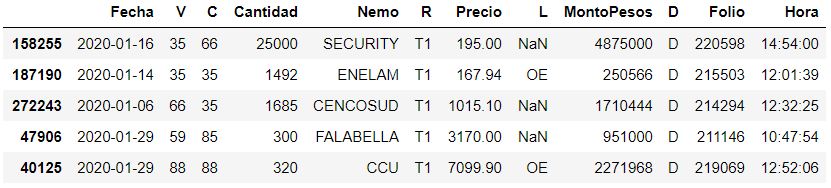
\includegraphics[scale=.5]{imgs/transacciones_RV_data.png}
   		\caption{Muestra de tamaño $5$ de datos disponibles para estimación del IPSA, transacciones en la bolsa durante enero $2020$.}
   		\label{fig:trans}
   	\end{figure}
   \begin{remark}
   	La mayoría de los datos financieros no incluyen fechas que correspondan a fines de semana o festivos. Esto se debe a que las instituciones que generan o recolectan estos datos no trabajan en tales días.
   \end{remark}
   	En la Figura \ref{fig:trans}, la columna \textit{Folio} identifica unívocamente a cada transacción, \textit{Precio} indica el precio al cual se transó,  \textit{Cantidad} la cantidad de acciones transadas, \textit{MontoPesos} corresponde a la multiplicación de las dos anteriores y \textit{Nemo} es la etiqueta que se le da a la acción en la bolsa, generalmente corresponde al nombre de la empresa que emite la acción. Algunos de estos Nemos son: BSANTANDER, FALABELLA y ENELCHILE, por ejemplo. El resto de las columnas no será relevante para este estudio.\\
   	Posteriormente, el valor del IPSA, $(X_t)_t$, lo aproximamos con la siguiente fórmula,
   	\begin{align}
   		\label{eq:ipsa1}
		X_t = base*\sum_{i\in I} w_i P(i)_t\\
		\label{eq:ipsa2}
		w_i = \frac{C_i}{\sum_{i\in I} C_ip(i)_0}
   	\end{align}
   donde $I$ es el conjunto de instrumentos que componen el IPSA el año $2020$ \footnote{\href{https://www.rankia.cl/blog/analisis-ipsa/3229498-que-empresas-forman-parte-ipsa-2021}{Lista de empresas componentes del IPSA $2020$ y $2021$.}}, $t$ hace referencia a días, $P(i)$ es la serie de precios diarios del instrumento $i$, $base$ corresponde al valor que se le quiera dar a la serie en tiempo inicial y $C_i$ es el número de acciones suscritas pagadas del instrumento $i$. Este último término se define como la parte de las acciones disponibles para la venta, y por ende para la obtención de fondos por parte de la empresa o sociedad que las emite, que efectivamente han sido suscritas y pagadas. En otras palabras, nos habla del tamaño de cada emisor en el mercado bursátil chileno.\\
   Por otra parte, notar que los \comillas{pesos} $w_i$ no suman $1$, sino que son tales que $X_0=base$. La Fórmula \ref{eq:ipsa1} no es la forma exacta del IPSA, esta busca aproximar el valor real usando los datos entregados por \textbf{LVA}.
   	\begin{remark}
   		El análisis no estuvo exento de daños en los datos. Las primeras aproximaciones al IPSA se caracterizaban por \textit{peaks} severamente pronunciados o fechas en las cuales los valores obtenidos simplemente no tenían sentido. Estos problemas se deben a que en el caso de no tener el dato, este era sustituido por $-1000$ y además, existe un rango de fechas, específicamente en el mes de marzo del $2020$, en las cuales los datos no fueron recolectados correctamente (ver Figura \ref{fig:danados}). Esta situación fue confirmada por el supervisor y se decide simplemente eliminar estas filas problemáticas. 
   		
   		\begin{figure}[H]
   			\centering
   			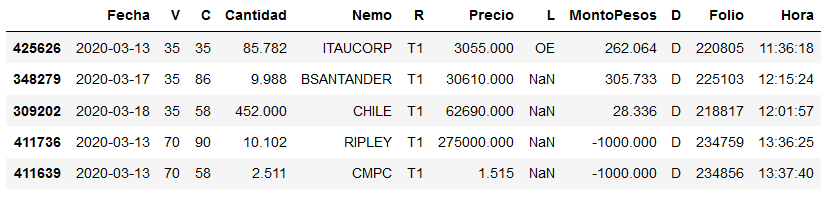
\includegraphics[scale=.5]{imgs/muestra_danada.png}
   			\caption{Muestra de datos dañados. Podemos ver los $-1000$ y que, por ejemplo, en la fila del $18$ de marzo del $2020$ la columna \textit{MontoPesos} claramente no corresponde a la multiplicación entre \textit{Cantidad} y \textit{Precio}.}
   			\label{fig:danados}
   		\end{figure}
   		
   	\end{remark}
   	
   	Lo primero que se necesita es estimar el precio de una acción en un día cualquiera. Para esto nos fijamos en una acción (o Nemo) y fecha cualquiera, a modo de ejemplo tomamos \textbf{CCU} y el $15$ de abril del $2020$. Para este par existen $456$ transacciones (ver Figura \ref{fig:ccu_abril}).   
   	\begin{figure}[H]
   		\centering
   		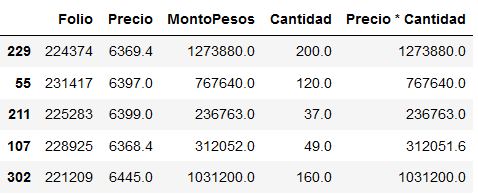
\includegraphics[scale=.5]{imgs/ccu_abril.png}
   		\caption{Muestra de tamaño $5$ de las transacciones asociadas a \textbf{CCU} el 15 de abril del $2020$.}
   		\label{fig:ccu_abril}
   	\end{figure}
   	Se decide calcular el precio del día como un promedio de los valores \textit{Precio} ponderando por los \textit{MontoPesos}. Es decir, para un instrumento $i$,
   	\begin{align*}
   		P(i)_t = \frac{1}{\sum_{k\in T(i,t)} MontoPesos_k}\sum_{k\in T(i,t)} Precio_k * MontoPesos_k
   	\end{align*}
 	donde $T(i,t)$ son las transacciones del instrumento $i$ en el día $t$. Lo anterior nos entrega una estimación del precio del día. Por otro lado, la cantidad de acciones suscritas pagadas la obtenemos de la página web de la \textit{Bolsa de Santiago} \footnote{\href{https://www.bolsadesantiago.com/}{Bolsa de Santiago.}}. Finalmente, en la Figura \ref{fig:ipsa_replication} se expone el resultado de este procedimiento.
	\begin{figure}[H]
		\centering
		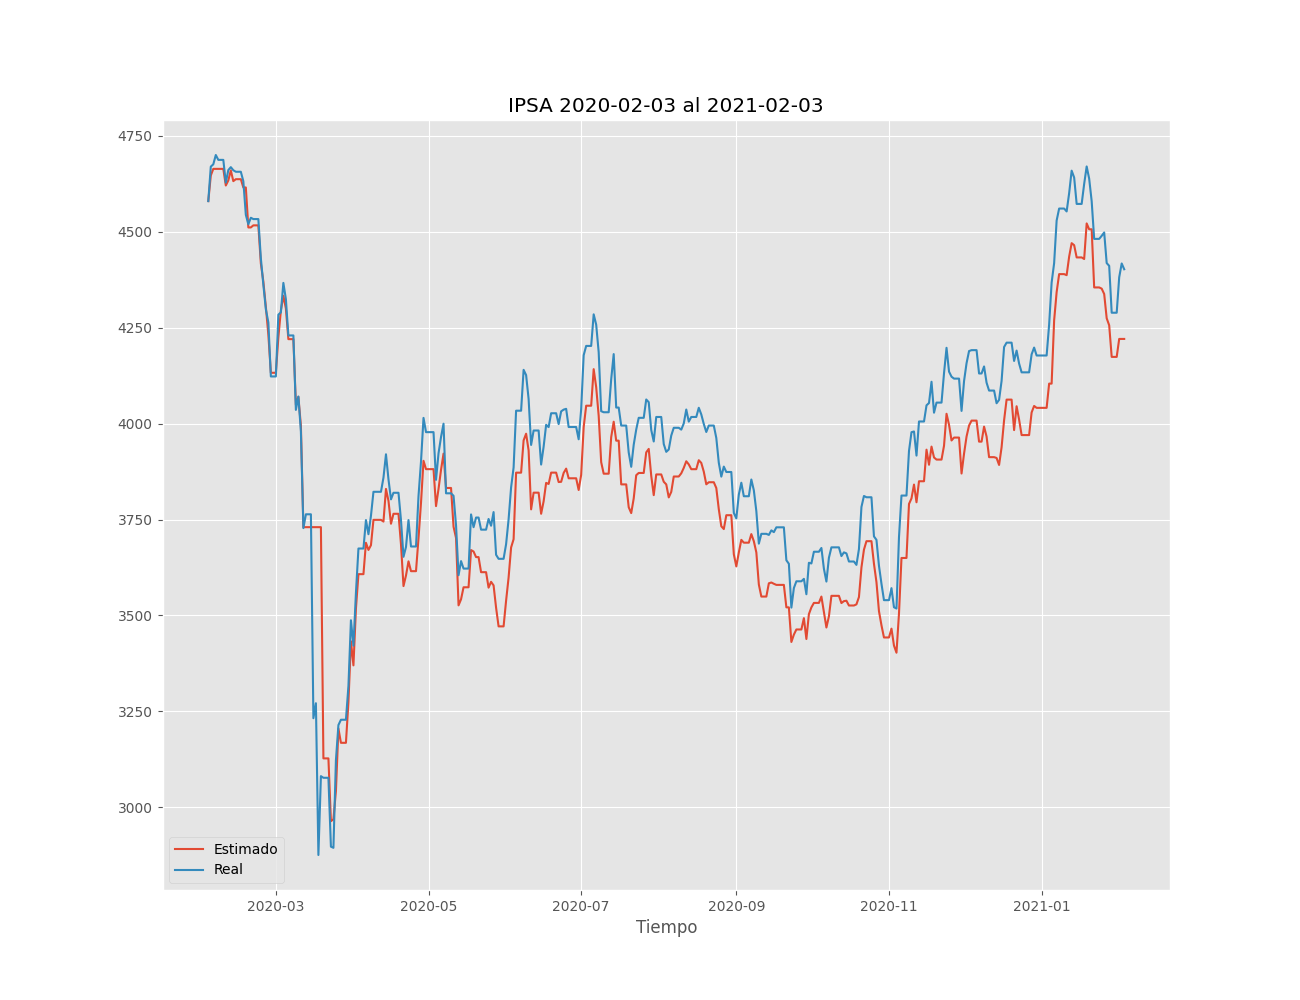
\includegraphics[scale=.5]{imgs/ipsa_replication.png}
		\caption{Replicación del IPSA.}
		\label{fig:ipsa_replication}
	\end{figure}
	La curva estimada captura bastante bien el comportamiento de la real, las subidas y bajadas del \textbf{IPSA} son logradas con buenos resultados. No obstante, es evidente el desfase que desde aproximadamente mediados de marzo comienza a hacerse notar y sigue la misma tendencia durante todo el periodo restante. Esta desviación se adjudica a la cantidad de datos dañados durante el periodo mencionado, ocasionando la recta horizontal en el punto donde el desfase comienza a hacerse más notorio. Por otro lado, es clara a la vista la caída que sufre el índice, tanto el real como el estimado, durante el mes de marzo. Esto refleja el esperado retroceso económico generado por la pandemia y no solamente en índices nacionales, la mayoría de los indicadores económicos mundiales sufrieron una caída similar.

\subsection{Monto óptimo}
	La segunda tarea requerida puede entenderse de forma independiente al objetivo principal de la práctica. Se cuenta con dos fuentes de datos, la primera es relativa a fondos mutuos y cada fila de esta tabla se interpreta como inversiones que realizan los distintos fondos en ciertas acciones y bonos (ver Figura \ref{fig:ffmm_data_sample}). La segunda corresponde a las transacciones que se realizan en la bolsa y da cuenta de cómo se mueve el mercado bursátil (ver Figura \ref{fig:trans}).
	\begin{figure}[H]
		\centering
		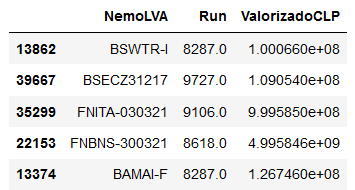
\includegraphics[scale=.65]{imgs/ffmm_data_sample.png}
		\caption{Muestra de tamaño $5$ de los datos de fondos mutuos.}
		\label{fig:ffmm_data_sample}
	\end{figure}
	Se busca generar un gráfico donde $x$ e $y$ representan la cantidad de transacciones e inversiones respectivamente que cumplan cierto criterio parametrizado por un monto $m$. Para el eje $Y$,  se agrupa la data de FFMM por run y luego por nemo para después sumar la columna \comillas{ValorizadoCLP} que tengan igual nemo dentro de cada grupo con el mismo run. Luego, dado un monto $m$, se cuenta la cantidad de inversiones resultantes (o intrumentos/nemos) tales que su monto sea menor a $m$ obteniendo un número $y$. Por otro lado, para el eje $X$, se agrupa la data por día y luego por nemo para despúes contar las inversiones que tengan igual nemo dentro de cada fecha. Después, para cada día se calcula la cantidad de transacciones que superen el monto $m$ para finalmente promediar este valor sobre un rango de días obteniendo la coordenada $x$.
\subsection{Datos de Twitter}
%En esta subsección se explicará el proceso de obtención de datos de Twitter y se muestra un pequeño análisis
Necesitamos analizar texto que represente una crítica o reseña sobre una compañía. Estos textos vendrán en forma de \textit{tweets} y queremos que hayan sido creados en cierto rango de fechas y que tengan ciertas palabras claves. Se investigaron variadas formas de hacer esto en \texttt{Python} pero se prefirió la librería \texttt{twint}\footnote{\href{https://github.com/twintproject/twint}{Repositorio de twint.}} dada su facilidad de uso y porque cuenta con la opción de manejar los tweets con DataFrames de \texttt{pandas}. Para obtener tweets con esta librería se debe especificar un intervalo de fechas y una request, esto último consiste en palabras claves o ciertas características que deban cumplir los tweets a buscar, ver Figura \ref{fig:twint_example}.
\begin{figure}[H]
	\centering
	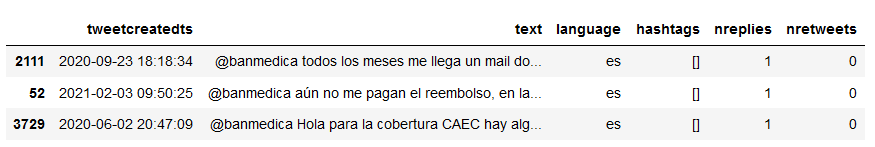
\includegraphics[scale=.65]{imgs/twint_example.png}
	\caption{Muestra de tamaño $3$ de \textit{tweets} obtenidos con \texttt{twint} con la request \comillas{@banmedica -from:banmedica}, esto significa que \texttt{twint} buscará tweets que etiqueten a Banmedica y que no vengan de la misma cuenta de Banmedica, más adelante se justificará esta request. La librería nos entrega un DataFrame con más columnas pero estas no fueron consideradas en este análisis.}
	\label{fig:twint_example}
\end{figure}
Se procede entonces a obtener tweets relativos a cada nemo o empresa del IPSA durante el periodo del $28$ de febrero del $2020$ y el $30$ de diciembre del mismo año, cabe señalar que esto tomó una cantidad de tiempo considerable obteniendo aproximadamente $1$\texttt{GB} de datos en archivos \texttt{.csv}. Se decide que la request para cada nemo sea de la forma \comillas{[cuenta(s) de la empresa] -from [cuenta(s) de la empresa]}, esto quiere decir que twint buscará tweets que etiqueten a la empresa en cuestión, con la idea de buscar reseñas o opiniones sobre esta, pero no buscará tweets que vengan de la empresa, esto para evitar posibles sesgos que vengan de la compañía.
\begin{remark}
Dado que algunas de las empresas asociadas a los nemos tenían una presencia relativamente baja en twitter, se decide por eliminarlas y trabajar solamente con las empresas cuyo promedio de tweets diarios sea mayor a $10$. El haber o no eliminado estos nemos no tiene efecto en el resultado final, veremos que las empresas escogidas para entrar al índice son siempre del grupo que tiene mayor presencia en la red social.
\end{remark}
\begin{figure}[H]
	\centering
	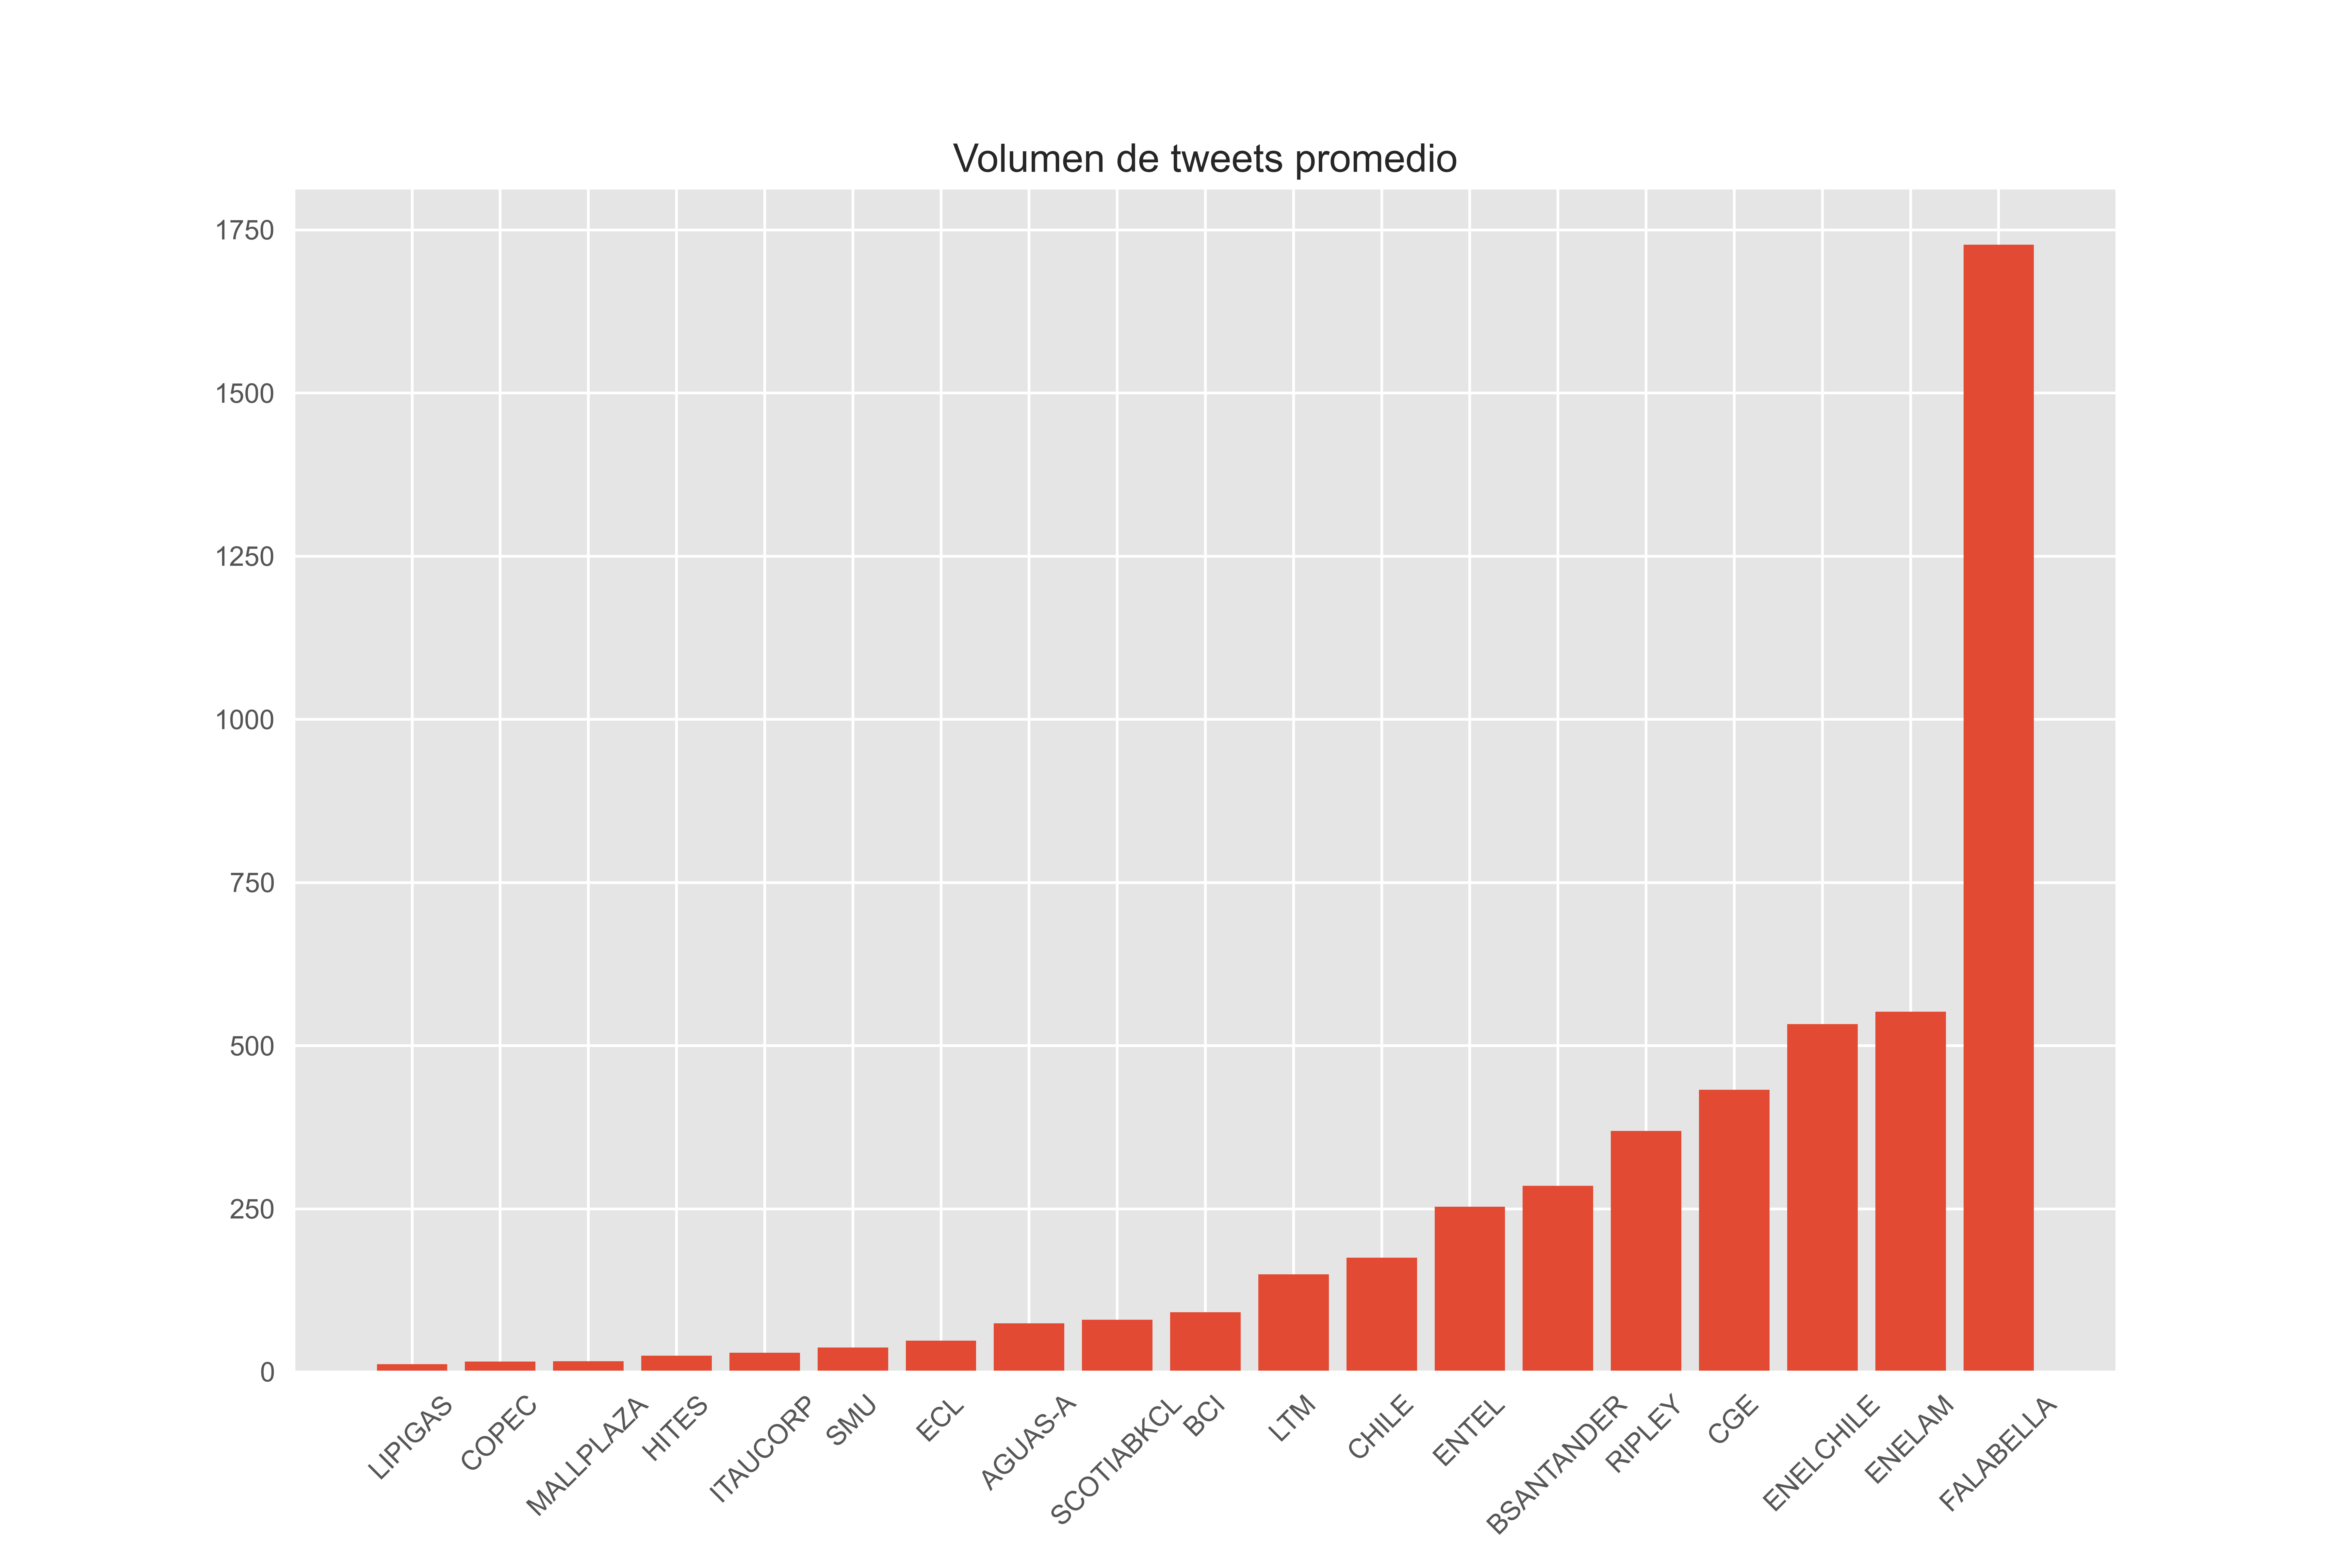
\includegraphics[scale=.38]{imgs/volume_tweets_agg.png}
	\caption{Promedio de tweets diarios relativos a las empresas con mayor presencia en la red social}
	\label{fig:volume_tweets_agg}
\end{figure}
La Figura \ref{fig:volume_tweets_agg} nos confirma que las empresas de retail, bancos, compañías de energía y agua son las más mencionadas en Twitter. Por el lado de las compañías de servicios básicos, cada vez que sucede un corte de agua o luz, las cuentas de estas empresas son mencionadas aumentando su volumen de tweets. Los bancos por otro lado, mantienen cuentas de tipo servicio al cliente y por lo tanto son constantemente mencionadas, tanto para dar críticas como para realmente preguntar por sus servicios. Finalmente, el caso del retail lo tenemos representado en gran parte por Falabella, esta es una de las compañías más grande en Chile (confirmado en parte por la Figura \ref{fig:volume_tweets_agg}) y además, debido a la pandemia, han aumentado la cantidad de compras online aumentando a su vez su presencia en redes sociales.
\begin{figure}[H]
	\centering
	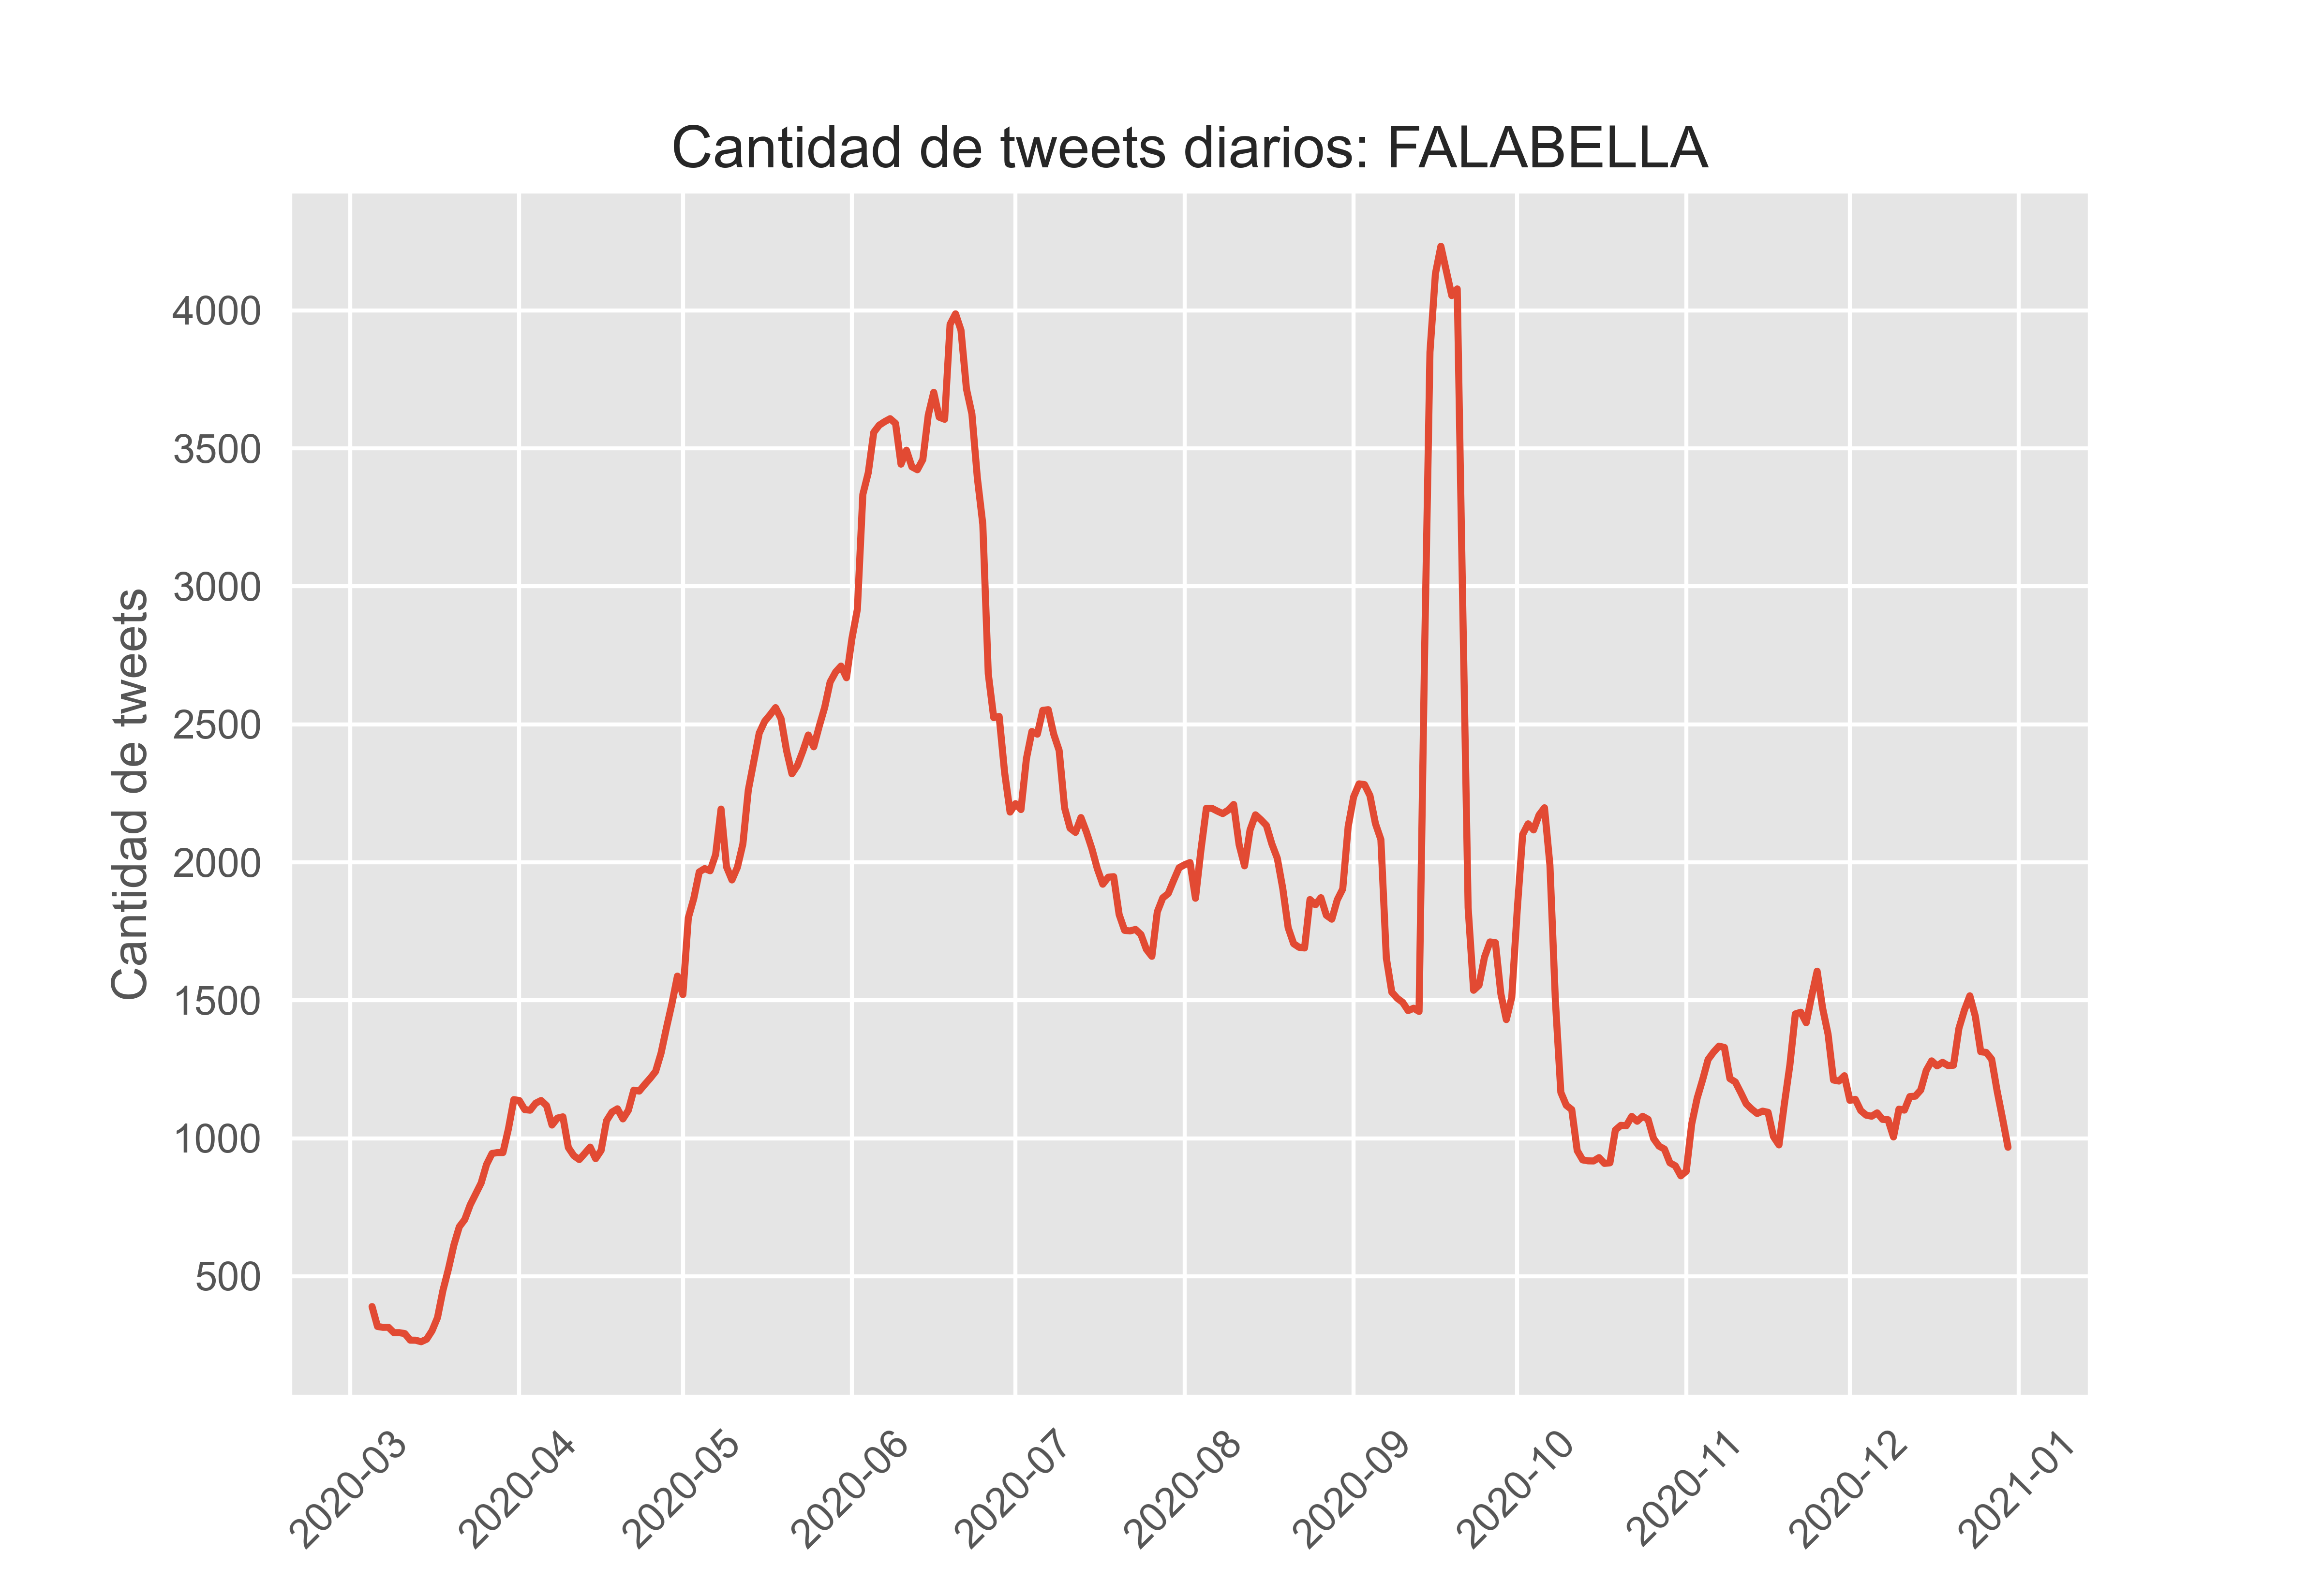
\includegraphics[scale=.55]{imgs/falabella_volume.png}
	\caption{Cantidad de tweets diarios mencionando a Falabella. Se toma un promedio móvil con ventana de $7$ días.}
	\label{fig:falabella_volume}
\end{figure}
\begin{figure}[H]
	\centering
	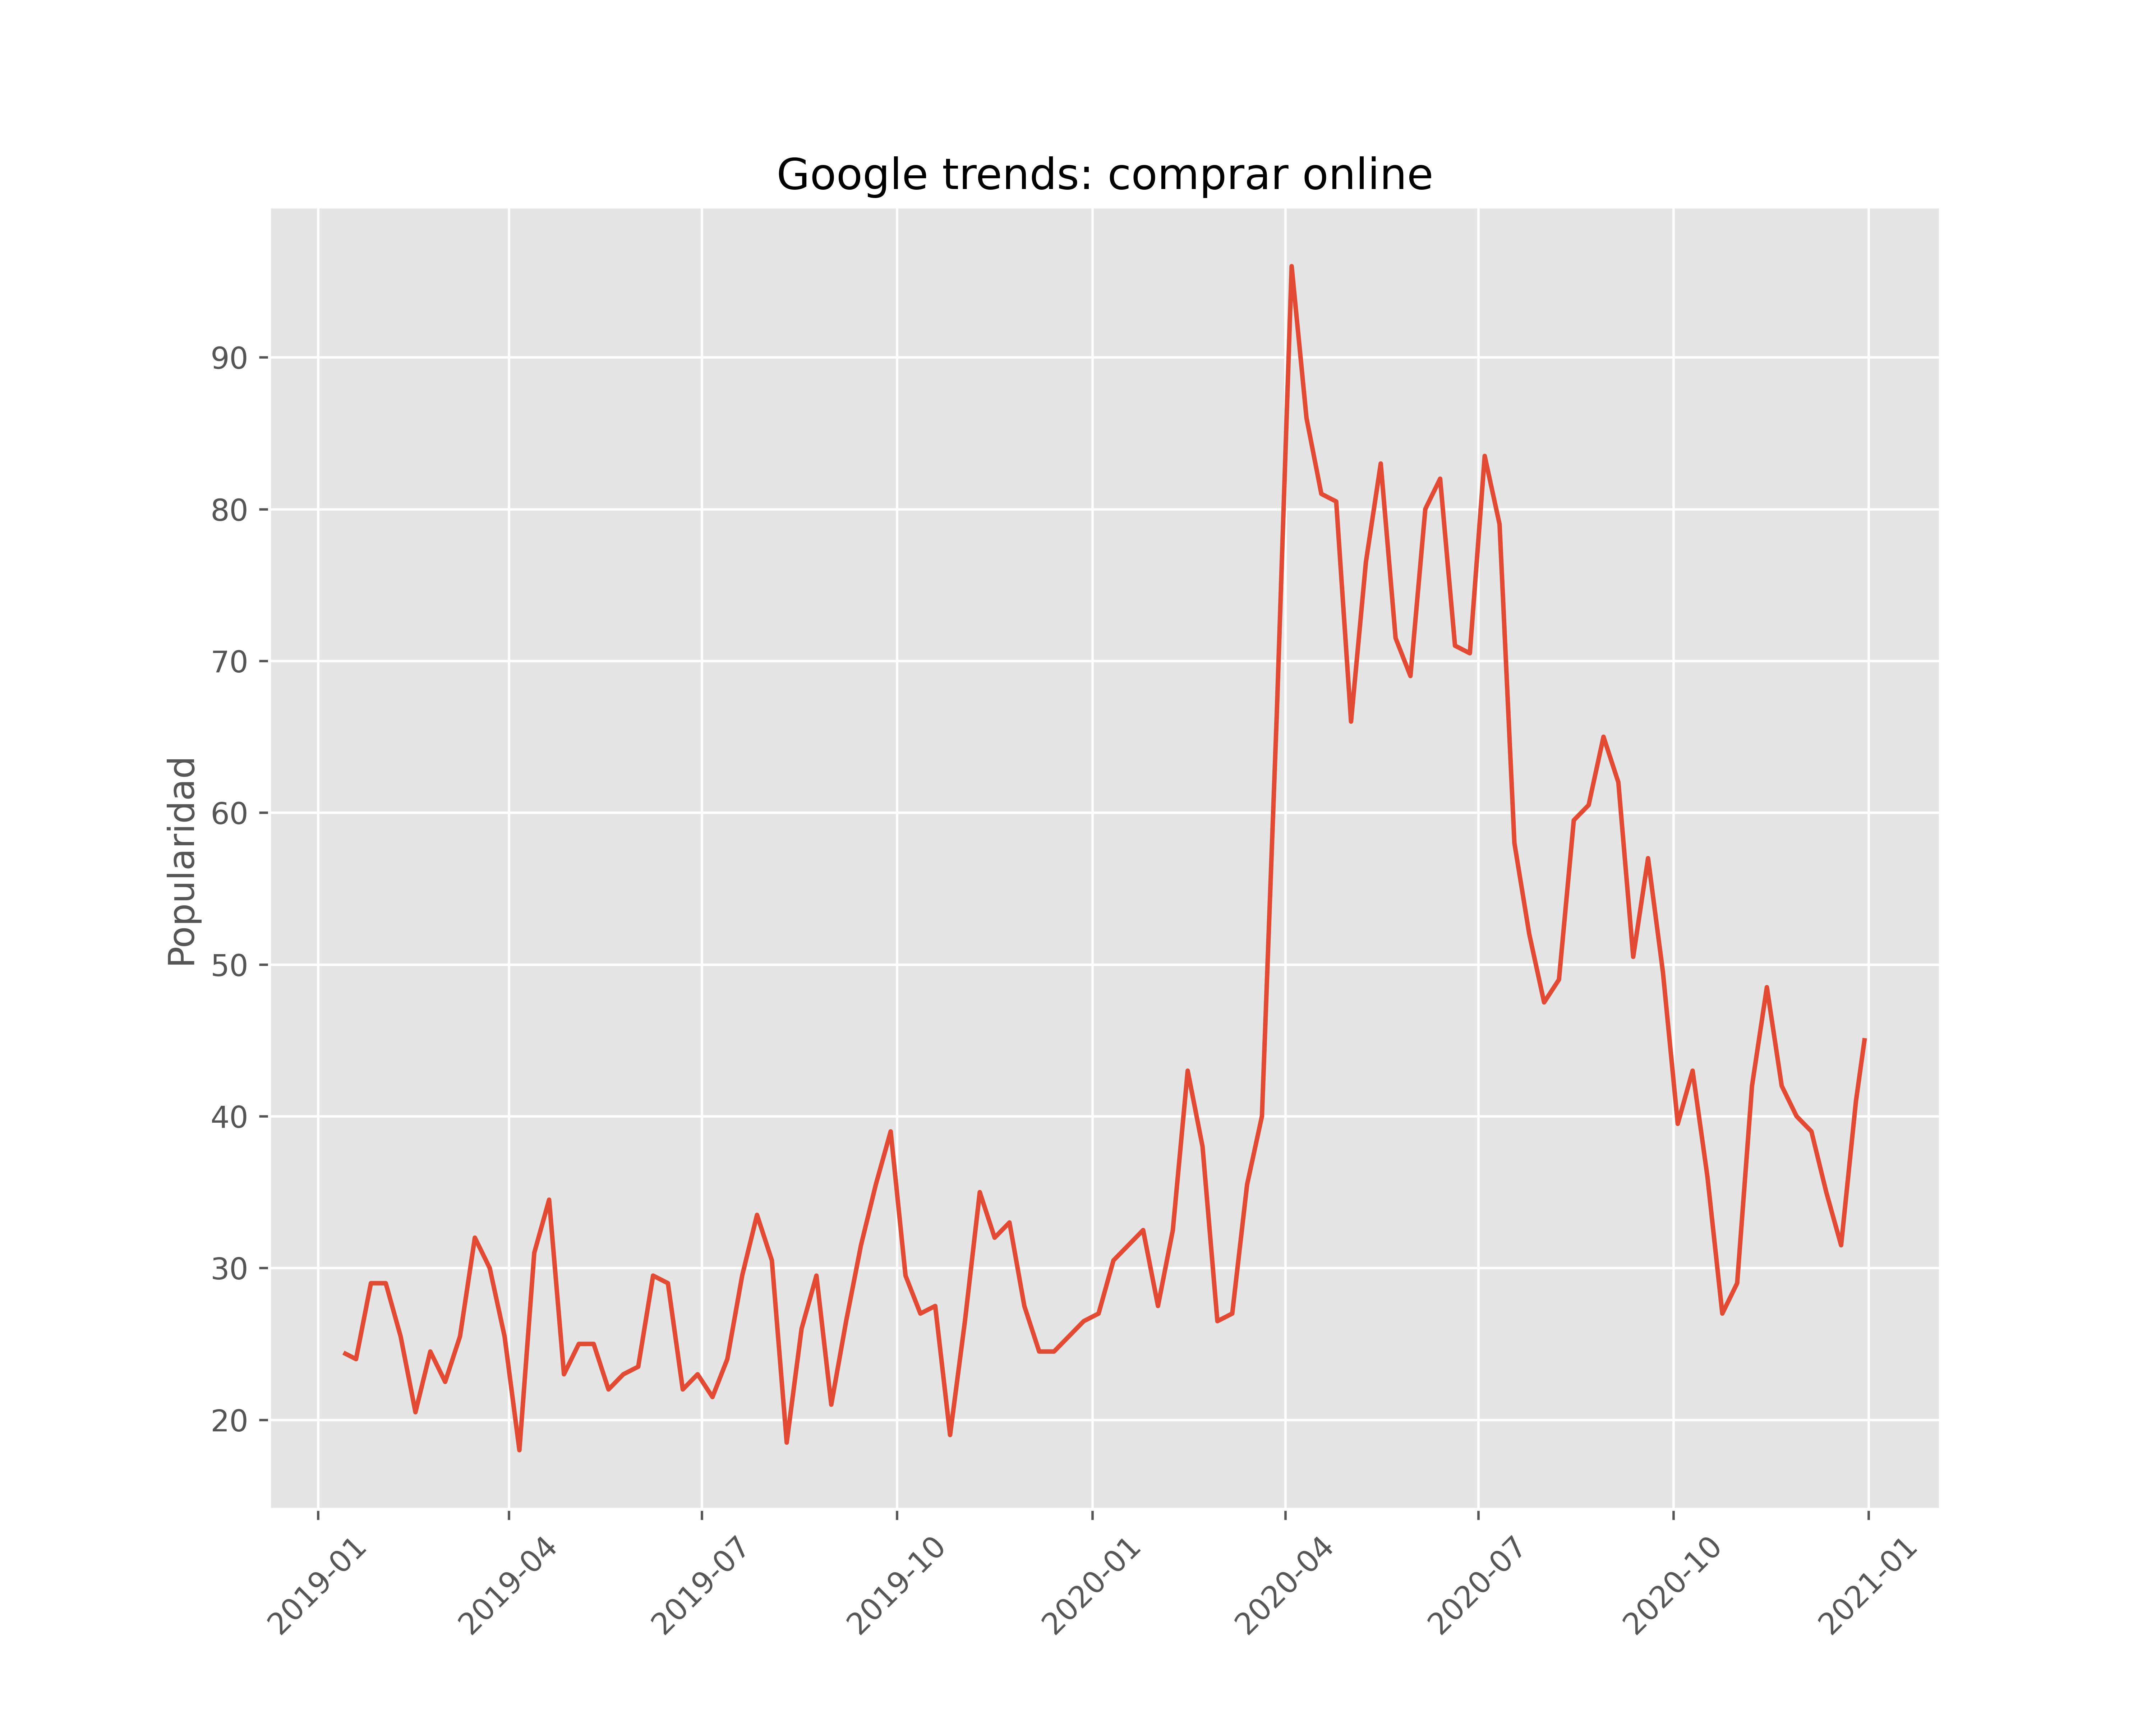
\includegraphics[scale=.42]{imgs/google_trend_compra_online.png}
	\caption{Popularidad del término de búsqueda \comillas{comprar online} en \href{https://trends.google.es/trends/?geo=CL}{Google trends} en Chile. Google define la popularidad como \comillas{el interés de búsqueda en relación con el valor máximo de un gráfico en una región y un periodo determinados}}
	\label{fig:google_trend_compra_online}
\end{figure}


En las Figuras \ref{fig:falabella_volume} y \ref{fig:google_trend_compra_online} se observa el comportamiento sugerido anteriormente, la presencia de Falabella en Twitter comienza a crecer durante los meses de marzo y abril, meses que coinciden con el inicio de la pandemia y además, como es de esperarse, el término \comillas{comprar online} aumenta su popularidad durante mismo periodo.



\subsection{Análisis de sentimiento}
El análisis de sentimientos corresponde a una parte del \textbf{NLP} (Natural Language Processing), la tarea de este es asignar a un trozo de texto un número que indique el puntaje del texto en cada sentimiento, esto son: negativo, neutro y positivo. La primera dificultad es que la mayoría de las librerías utilizadas para esta tarea están hechas para analizar textos en inglés, al investigar la existencia de análogos en español, se llega a la librería \texttt{pysentimiento}, ver Figura \ref{fig:pysentimiento_example}.\\
\begin{figure}[H]
	\centering
	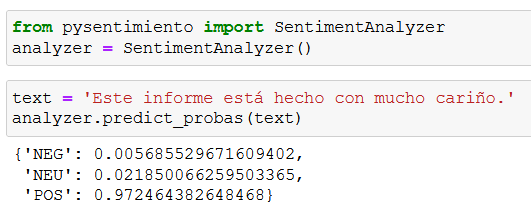
\includegraphics[scale=.65]{imgs/pysentimiento_example.png}
	\vspace{.5cm}
	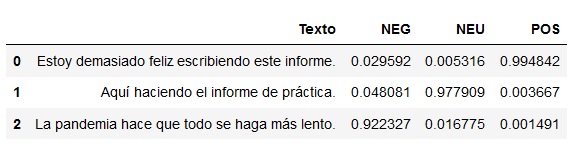
\includegraphics[scale=.65]{imgs/pysentimiento_example2.png}
	\caption{Ejemplos de uso de la librería \texttt{pysentimiento}.}
	\label{fig:pysentimiento_example}
\end{figure}
\subsection{Creación del índice}
En esta subsección se mezclan las herramientas de las partes anteriores para implementar un programa que obtenga tweets asociados a cada nemo, analice sus sentimientos y maneje toda la información con DataFrames de \texttt{pandas}. A grandes rásgos, la lógica del código se hizo en base a una jerarquía de clases simple, esta consiste en una clase madre \texttt{Instrument} que representa un instrumento financiero genérico y clases \texttt{InstrumentRV} e \texttt{InstrumentRF} que heredan de la anterior y representan respectivamente a acciones y bonos. El tratamiento de bonos resulta un poco más complicado y será reportado más adelante en el informe. 
\begin{figure}[H]
	\centering
	%\tikzstyle{block} = [rectangle, draw, fill=blue!20, text centered]
\begin{center}
	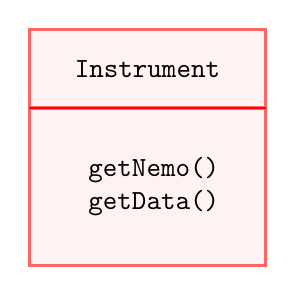
\begin{tikzpicture}
		%\node [block] (madre) {Instrument};
		%\node [block, below of=madre] {InstrumentRV};
		% Cajas
		\filldraw[color=red!60, fill=red!5, very thick] (0,0) rectangle (3,2);
		\filldraw[color=red!60, fill=red!5, very thick] (0,2) rectangle (3,3);
		\draw[thick, red, -] (0,2) -- (3,2);
		% Tamaños de las cajas
		\node[] at (1.5,2.5) {\texttt{Instrument}};
		\node[text width=1.5cm,text centered] at (1.5,1) {
			\texttt{getNemo()}
			\texttt{getData()}
		};
		% Aristas
		
		%\draw[thick,red,-] (1.5,0) -- (4.5,0) ;
		
		% Cajas
		%\node [draw, thick, shape=rectangle, minimum width=3cm, minimum height=3cm, anchor=center, color=blue] at (0,0) {};
		%\node [draw, thick, shape=rectangle, minimum width=3cm, minimum height=3cm, anchor=center, color=blue] at (6,0) {};
	\end{tikzpicture}
\end{center}
	\caption{Resumen diagrama UML del código.}
	\label{fig:uml}
\end{figure}
El input del programa consiste en un diccionario, digamos \texttt{dict}, tal que \texttt{dict[\comillas{RV}]} y \texttt{dict[\comillas{RF}]} entreguen, correspondientemente, la lista de nemos de acciones y bonos considerados para trabajar en el índice. Idealmente este diccionario guarda todos los instrumentos del mercado chileno, pero dado que no todos estos tienen presencia destacable en redes sociales, se trabaja sólo con un subconjunto del total de instrumentos. Las acciones consideradas son un subconjunto de las acciones que conforman el IPSA y los bonos son los que tienen registro en las bases de datos de LVA y que sean emitidos por compañías con presencia destacable en twitter, esto último hace que existan empresas relacionadas tanto a bonos como acciones y nemos de bonos asociados a la misma empresa. Para solucionar este enredo se crea un diccionario auxiliar que relaciona cada emisor de bonos a una lista de nemos que este emite, luego, se recorre el diccionario de emisores creando los objetos correspondiente como \texttt{InstrumentRF(nemo, emisor)}. El caso de las acciones es más simple dado que, por lo menos en este contexto, hay una relación uno a uno entre empresas y nemos de acciones. En esta parte del programa se cuenta con una lista de objetos tipo \texttt{Instrument} a los cuales se les \comillas{setean} sus datos con el método \texttt{setData()}. Dado que por cada día se tienen varios tweets, el valor de las columnas neg, neu y pos en el dataframe de la Figura \ref{fig:instrument_sentiment_sample} corresponde al promedio de estos valores en los tweets del día.\\
\begin{figure}[H]
	\centering
	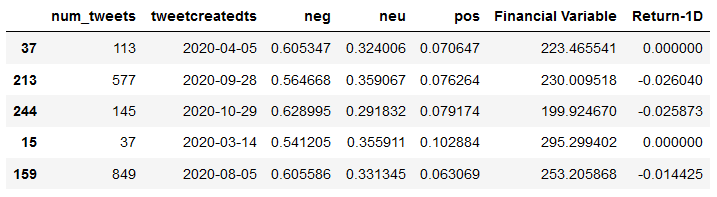
\includegraphics[scale=.65]{imgs/instrument_sentiment_sample.png}
	\caption{Dataframe asociado al \texttt{InstrumentRV} que representa a COPEC.}
	\label{fig:instrument_sentiment_sample}
\end{figure}


\begin{figure}[H]
	\centering
	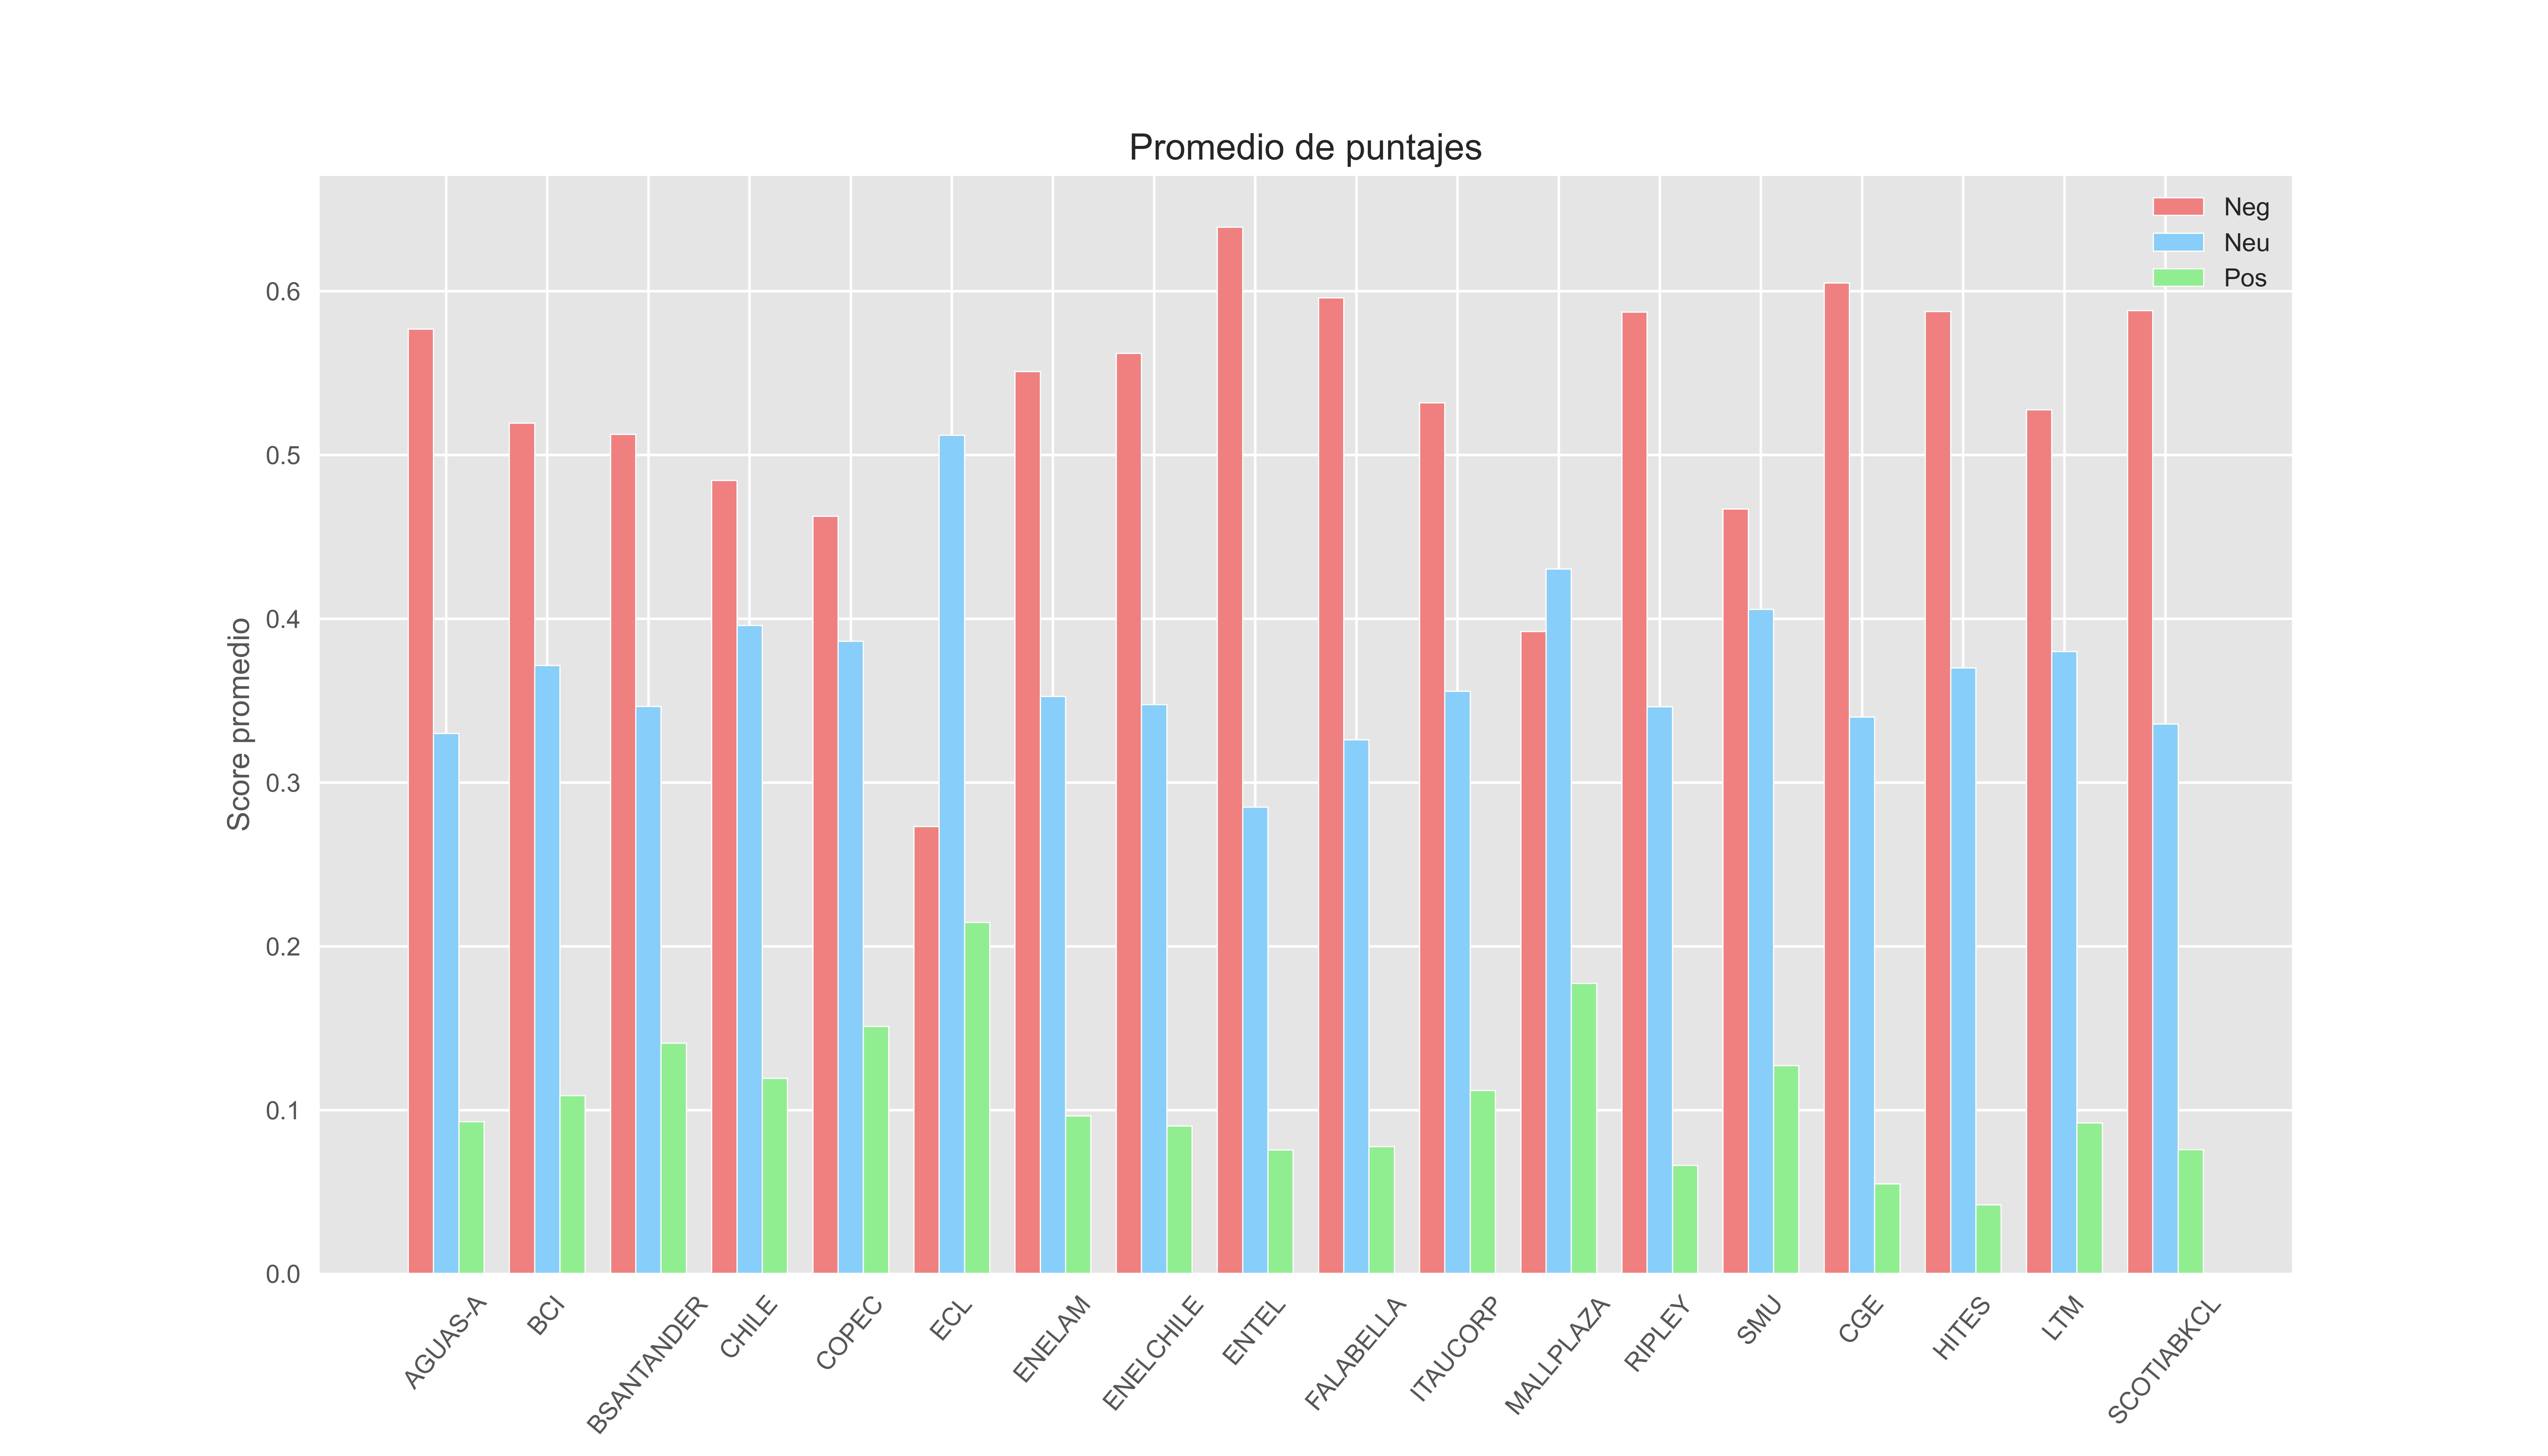
\includegraphics[scale=.45]{imgs/mean_score_bar.png}
	\caption{Promedio de los score en cada sentimiento para las acciones con mayor presencia en Twitter.}
	\label{fig:mean_score_bar}
\end{figure}

La Figura \ref{fig:mean_score_bar} nos ratifica la sospecha que se tenía desde un principio y es que la mayoría de los tweets tienen carácter negativo con un score mayor a $0.5$.
%%%%%%%%%%%%%%%%%% END DOCUMENT %%%%%%%%%%%%%%%%%%



\newpage

%\begin{thebibliography}{99}
	
\end{thebibliography}
\section{Punto de que hablar}
    \begin{enumerate}
        \item Calculo de índices: IPSA. Explicar el cálculo del índice y por qué se calcula este tipo de indicadores.
        \item Análisis de sentimientos con twitter: Hablar de la cantidad de data por nemo y poner gráfico de barras.
        \item Hablar de la decisión de dejar retweets porque representan el mismo comentarios pero de otra persona.
        \item Comentar que hay tweets en otros idiomas y por lo tanto se hizo necesario trabajar con APIs de idioma.
        \item Series de tiempo en economía.
        \item Correlación entre dos variables. 
        \item Test de correlación.
        \item Explicar el cálculo del sentimiento saturado, shifted y todo el preproceso que se le hace a los valores pos, neu y neg para transformarlos en un número representativo del sentimiento de cada tweet
        \item Explicar que el sentimiento del día asociado a un instrumento se calcula como un promedio de los score de tweets diarios.
        \item Explicar que se busca parámetros que maximicen la correlación entre las variables adecuadas: \textbf{retorno} del sentimiento, sentimiento promedio en el periodo \textbf{sent days}, promedio de los retornos diarios, etc contra el retorno del precio de la acción o menos la tasa de interés para el caso de bonos.
        \item Mostrar los gráficos del índice obtenido y los nemos que participan del índice.
    \end{enumerate}


\end{document}
